\documentclass[../thesis]{subfiles}

\begin{document}
	\subsection{\nvidia Kepler Architecture}
	\label{subsec:cuda:arch:kepler}
	
	Kepler devices contain up to 15 \smx, an improved version of \sm, with more and smaller cores, working at half the clock frequency. L2 cache size was doubled to 1536 KB. Each individual \smx contains up to 192 cores and 64K registers, with a maximum number of registers per thread of 255. In comparison with older architectures like Fermi, the Kepler architecture adds a new 48 KB read-only data cache and a new 32KB+32KB configuration for the L1 cache and shared memory.

	Some of the new features of this architecture are mainly targeted at programming, such as the introduction of dynamic programming and Hyper-Q. Dynamic programming allows the device to generate work for itself, therefore enabling it to adapt to the amount and form of parallelism throughout the program's execution. Hyper-Q enables the cores from the same \cpu to launch kernels in the same \gpu. Multiple kernels launched in the same \gpu will be scheduled to different \smx.

	Load units in the Kepler architecture are capable of getting blocks of 256 bytes from shared memory \cite{NVIDIA:KEPLER}.

	\begin{figure}[p]
		\addtolength\belowcaptionskip{1cm}
		\caption{Overview of the Kepler GK110 architecture}
		\addtolength\belowcaptionskip{-1cm}
		\label{fig:gk110}
		\begin{subfigure}[t]{\textwidth}
			\centering
			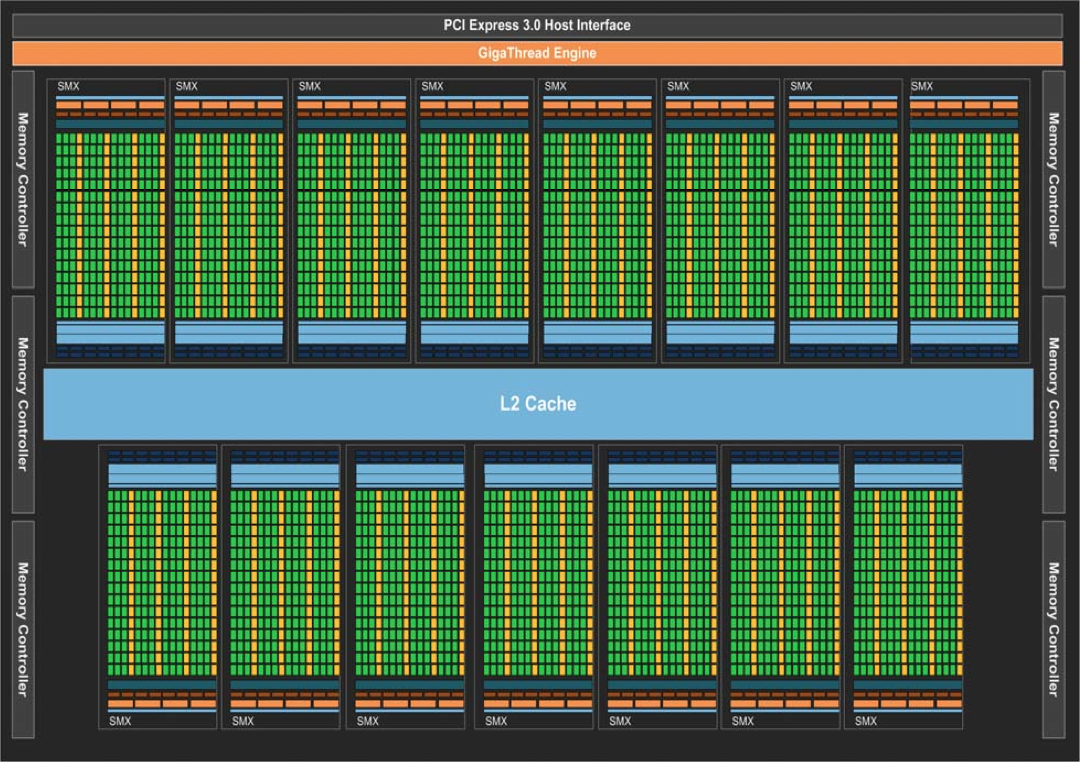
\includegraphics[height=0.4\textheight]{assets/images/cuda/arch/gk110.png}
			\addtolength\belowcaptionskip{0.5cm}
			\caption{Full chip block diagram}
			\addtolength\belowcaptionskip{-0.5cm}
		\end{subfigure}
		\begin{subfigure}[b]{\textwidth}
			\centering
			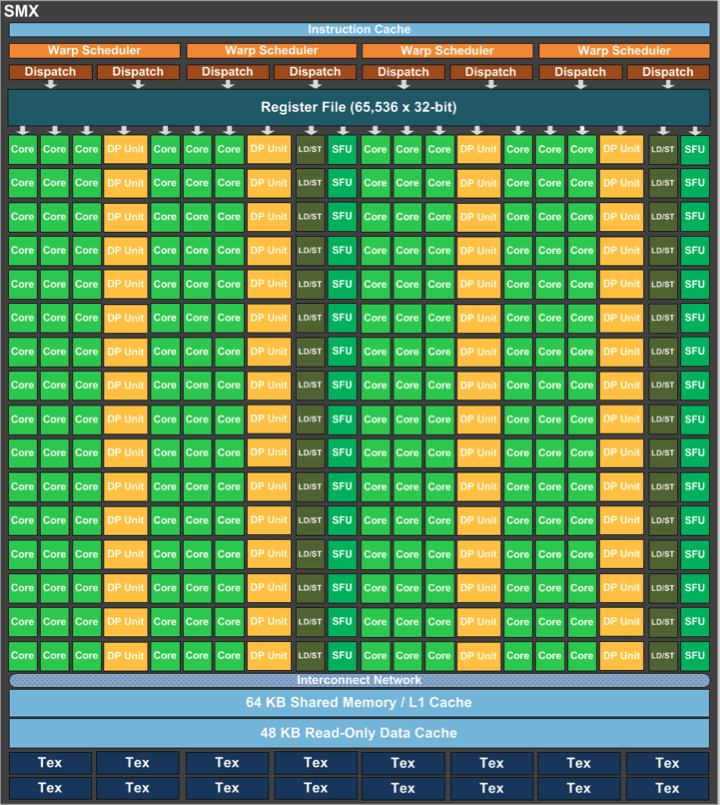
\includegraphics[height=0.4\textheight]{assets/images/cuda/arch/smx.png}
			\caption{\acs{SMX} diagram}
		\end{subfigure}
	\end{figure}
\end{document}
